\documentclass[11pt,a4paper]{article}
\usepackage{import}
\subimport{../../shared/}{preamble.tex}
\addbibresource{bibliography/references.bib}
\title{Torque-Referenced Consistency Regularization of dq Flux Maps}
\author{}
\date{7 October 2026}
\newcommand{\PaperAbstract}{Can an independently measured stationary torque expose and reduce spatially implausible structure in a reconstructed dq flux map? We model measured-minus-predicted torque as an unknown group offset plus spatial structure and noise; agreement therefore means a nearly flat residual within comparable speed, temperature and configuration, not pointwise equality. This yields a global minimum-change and smoothness-regularized flux correction. A scalar co-energy correction is used as the physically motivated numerical variant because it enforces reciprocity structurally, while remaining a prior rather than proof of magnetic truth. In a known-truth experiment it reduces flux RMSE and centered torque-residual spread; an injected radial potential remains invisible, as predicted by the retained rank-one observability theory. A portable two-system PSM dataset demonstrates offset removal and multi-speed transfer checks with $k_T=3p$. The CAN channel, shaft losses, terminal-current reconstruction and speed-dependent nuisance mechanisms remain experimentally unqualified, so no true-flux claim is made.}
\newif\ifshowglossary\showglossarytrue
\newif\ifshowbibliography\showbibliographytrue


\begin{document}
\maketitle
\begin{abstract}
\PaperAbstract
\end{abstract}
\tableofcontents


\section{Question: what does torque actually tell us about a flux vector?}
The familiar dq torque equation is usually used in the forward direction: flux and current predict torque. For flux-map validation the inverse question is more revealing. Given current and an independent torque observation, which part of the two-dimensional flux vector has actually been measured?

The answer is a projection, not a complete reconstruction. This paper develops that geometry, derives the corresponding solution line and minimum-change representative, and then asks whether magnetic reciprocity removes the missing direction. It does not: smooth radial potential terms remain invisible to torque. The synthetic and conditional real-data studies are organized around this observability statement. Co-energy fitting and general measurement-error identification are deliberately kept in separate papers.

\section{Stationary torque residual and its nuisance offset}
\label{sec:stationary-residual}
Under a declared dq scaling and phase-system configuration, a reconstructed
flux map predicts
\begin{equation}
 M_{\mathrm{theo}}=\kt(\psid\iq-\psiq\id).
 \label{eq:theoretical-torque}
\end{equation}
Define measured minus theoretical torque,
\begin{equation}
 \boxed{\stationarytorqueresidual=M_{\mathrm{meas}}-M_{\mathrm{theo}}.}
 \label{eq:stationary-residual}
\end{equation}
The sign matters: a positive flux correction that increases theoretical torque
decreases this residual. The measured channel must be independent of the voltage
signals used for flux reconstruction; independence of electronics does not by
itself establish calibrated electromagnetic truth.

At stationary mechanical speed the schematic rotor balance is
\begin{equation}
 \rotorinertia\dot{\mechanicalspeed}
 =M_{\mathrm{em}}-\shafttorque-\mechanicallosstorque,
 \qquad \dot\omega_{\mathrm m}\simeq0.
 \label{eq:stationary-balance}
\end{equation}
Mechanical friction and windage, sensor-chain offset and some nearly constant
loss contribution can therefore separate measured shaft torque from the
electromagnetic model. Iron loss is not generally constant across a current
map even at fixed speed: flux amplitude, saturation and harmonics vary with
operating point. Current-dependent mechanical or electrical loss and calibration
gain can likewise create structure. A constant offset is consequently a first
model level, not a law of the machine.

For a group $g$ with approximately equal speed, thermal state, excitation and
measurement configuration, write
\begin{equation}
 \stationarytorqueresidual(i_d,i_q)
 =\torquegroupoffset+\delta r_M(i_d,i_q)+\varepsilon.
 \label{eq:residual-decomposition}
\end{equation}
The nuisance offset $c_g$ is not a target for flux correction. The structured
part $\delta r_M$ is the diagnostic signal; $\varepsilon$ represents measurement
and reconstruction scatter. The first hypothesis is
\begin{equation}
 \boxed{M_{\mathrm{meas}}-M_{\mathrm{theo,corr}}\simeq c_g
 \quad\text{within each qualified group}.}
 \label{eq:flat-residual-hypothesis}
\end{equation}
A nearly constant nonzero residual is therefore a successful first-order
consistency pattern. If spatially cross-validated low-order residual structure
remains, the next model level is a slowly varying nuisance surface. It should be
introduced only after the constant model fails, and it must not silently absorb
the same high-frequency structure that the flux diagnostic is meant to test.

Algebraically, centering removes one scalar per group. Geometrically, it aligns
the vertical level of the two torque surfaces without changing their shape.
Physically, it tolerates unmodeled mean loss and offset. Experimentally, it
prevents a large harmless bias from dominating a spatial-consistency metric.

\section{From residual structure to a global flux correction}
\label{sec:global-regularization}
Let the corrected field be
\begin{equation}
 \flux_{\mathrm{corr}}=\flux_{\mathrm{raw}}+\Delta\flux,
 \qquad \Delta\flux=\begin{bmatrix}\Delta\psi_d&\Delta\psi_q\end{bmatrix}^{\mathsf T}.
\end{equation}
At a fixed current the torque change is
\begin{equation}
 \Delta M=\kt(\iq\Delta\psi_d-\id\Delta\psi_q),
\end{equation}
and hence
\begin{equation}
 r_{M,\mathrm{corr}}=r_{M,\mathrm{raw}}
 -\kt(\iq\Delta\psi_d-\id\Delta\psi_q).
 \label{eq:corrected-residual}
\end{equation}
Applying this equation independently at every point would reproduce noise and
choose an arbitrary member of a local solution line. The desired object is a
single field over the complete supported current domain. A general discrete
formulation is
\begin{multline}
 \min_{\Delta\flux,\{c_g\}}
 \sum_k w_k\left[r_{M,k}-c_{g(k)}
 -\kt(i_{q,k}\Delta\psi_{d,k}-i_{d,k}\Delta\psi_{q,k})\right]^2\\
 +\lambda_{\mathrm{smooth}}J_{\mathrm{smooth}}(\Delta\flux)
 +\lambda_{\mathrm{change}}J_{\mathrm{change}}(\Delta\flux)
 +J_{\mathrm{prior}}.
 \label{eq:global-objective}
\end{multline}
The data term flattens residual shape rather than forcing zero. Smoothness
couples neighboring operating points; change regularization keeps the raw map
unless torque provides enough evidence to move it. Weights can represent a
declared covariance, but repeat scatter is not automatically independent sensor
uncertainty. Bounds, parity or other physics enter through $J_{\mathrm{prior}}$
and must remain visible assumptions.
This data-fidelity-plus-penalty structure is generalized Tikhonov
regularization; the penalty encodes prior information rather than another
measurement \cite{hohage2020inverse}.

\subsection{Why the numerical experiment uses a co-energy correction}
A particularly coherent variant introduces one scalar surface,
\begin{equation}
 \Delta\coenergy(i_d,i_q),\qquad
 \Delta\psid=\partial_{i_d}\Delta W',\quad
 \Delta\psiq=\partial_{i_q}\Delta W'.
 \label{eq:coenergy-correction}
\end{equation}
Both components then come from one smooth potential and the mixed derivatives
are reciprocal by construction. Curvature regularization acts on the scalar
surface rather than coordinating two unrelated maps. The experiments use the
repository's gauge-fixed degree-four tensor B-spline basis and penalize its
third derivatives plus correction magnitude. No reflection parity is imposed.

This parameterization is used as a physically motivated variant of the general
objective, not as a theorem that the measured terminal-current field is a true
storage gradient. Torque alone does not determine radial co-energy, and a
conservative low-residual fit can still be physically wrong. The companion
integrability paper owns the admissibility tests; the companion reconstruction
paper owns general potential fitting. Here the potential basis supplies a
transparent global regularizer and a reproducible reciprocity prior.

The change and smoothness weights select a representative inside a large
feasible family. Sensitivity across $\lambda$ must therefore accompany any
reported correction. On real data, where true flux is unavailable, $\lambda$
cannot be selected by flux RMSE; the paper reports a fixed conservative example
and its path rather than optimizing against the same torque residual and calling
that validation.

\section{Torque observes one flux projection}
\label{sec:torque-observability}
\subsection{The question answered by a torque observation}
Reciprocity tests whether two flux surfaces can be slopes of one landscape.
It does not fix the height or all slopes of that landscape. An independent
mechanical observation poses a different question: which part of a local
flux vector contributes to electromagnetic torque? Under the amplitude-invariant
fundamental dq convention and a declared phase-system configuration, the relation is
\begin{equation}
 M_{\rm map}=\kt(\psid i_q-\psiq i_d).
 \label{eq:torque-flux}
\end{equation}
For one amplitude-invariant three-phase system $k_{\rm T}=3p/2$; two equally
represented systems give total $k_{\rm T}=3p$, as in the real experiment in
\cref{eq:dual-system-torque}. Throughout this derivation the factor is known
from the declared convention, not estimated from agreement. The same
convention must apply to both currents and fluxes
\cite{binder2017,schroeder2021,jebai2014}. With power-invariant scaling of
both vectors for one three-phase system the coefficient is instead $p$. A scaling change cannot be
applied to just one channel. In a loss-aware model one must also specify
which currents and fluxes enter the torque law; terminal samples are not
automatically storage coordinates.

Torque-assisted parameter identification is already used for SPMSMs;
Wang et al.\ combine torque and voltage information in a sensorless
parameter estimator \cite{wang2026torque}. Here the object is an arbitrary
nonlinear flux field and its observable directions, rather than a particular
parameter estimator. The following projection is an algebraic reformulation
of \cref{eq:torque-flux}, not a claim of an established new flux species.

For nonzero stator current introduce the unit current direction and its
clockwise normal:
\begin{equation}
 \statorcurrent=\begin{bmatrix}i_d\\i_q\end{bmatrix},\quad
 \statorcurrentmagnitude=\sqrt{i_d^2+i_q^2},\quad
 \currentunitdirection=\frac{\statorcurrent}{I_s},\quad
 \torqueunitdirection=\frac{-\rotationgenerator\statorcurrent}{I_s}
                    =\frac{1}{I_s}\begin{bmatrix}i_q\\-i_d\end{bmatrix}.
 \label{eq:torque-directions}
\end{equation}
The two unit directions are orthogonal. Decomposing the flux vector gives
\begin{equation}
 \flux=\currentparallelflux\currentunitdirection+
       \torqueobservableflux\torqueunitdirection,\qquad
 \psi_i=\vect n_i\trans\flux,\quad
 \psi_\tau=\vect n_\tau\trans\flux,\quad
 M_{\rm map}=k_{\rm T}I_s\psi_\tau .
 \label{eq:torque-projection}
\end{equation}
We refer to $\psi_\tau$ as the torque-observable flux component in the
following. It is a signed, current-dependent projection in Wb, not the
flux magnitude or a separate winding linkage. Torque is the oriented
area spanned by current and flux times $k_{\rm T}$: a parallel addition
changes no area, whereas a normal addition changes it directly.
\begin{figure}[tbp]
 \centering
 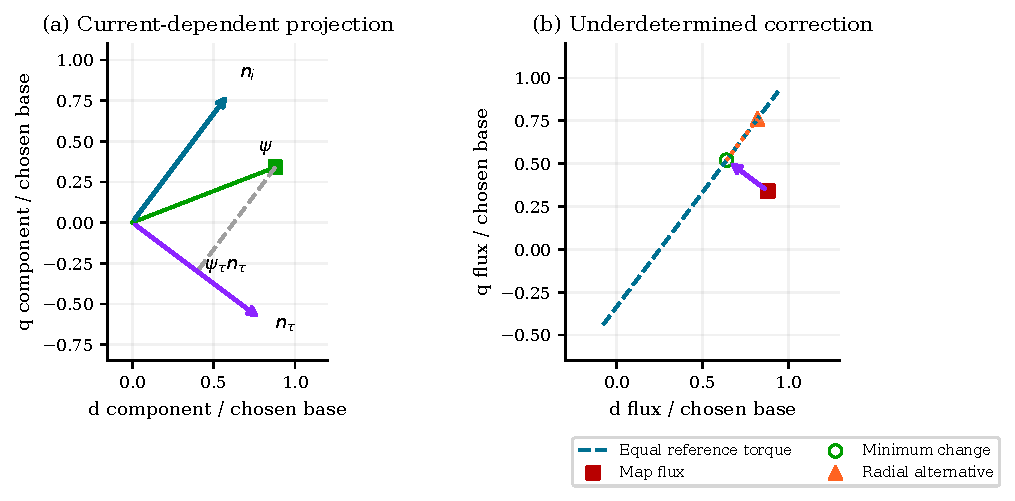
\includegraphics[width=\textwidth]{figures/06_torque_geometry.pdf}
 \caption{Local torque geometry in dimensionless coordinates. Left: a
 clockwise normal extracts the torque-producing projection; the dashed
 projection line is parallel to current. Right: a reference torque defines
 a line of admissible flux vectors. The arrow selects the closest vector;
 the triangular point adds an equally admissible radial change. Marker
 shapes and line patterns retain the distinction without color.}
 \label{fig:torque-geometry}
\end{figure}

For a qualified reference for the electromagnetic torque represented by
this model, define
\begin{equation}
 \psi_{\tau,\rm ref}=\frac{\electromagnetictorquereference}{k_{\rm T}I_s},
 \quad \torqueconsistencyresidual=M_{\rm map}-M_{\rm em,ref},
 \quad \torquefluxresidual=\psi_{\tau,\rm map}-\psi_{\tau,\rm ref}
                         =\frac{e_M}{k_{\rm T}I_s}.
 \label{eq:torque-residual}
\end{equation}
The normalized residual has flux units and compares the same observable
direction across current magnitudes. It does not attribute disagreement
to flux alone. If current is treated as exact and torque noise has standard
deviation $\sigma_M$, its contribution has
$\sigma_{\psi_\tau}=\sigma_M/(|k_{\rm T}|I_s)$. At zero current torque is
zero for every finite flux vector, the local rank becomes zero, and the
unit directions and normalized residual are undefined. A current threshold
must replace normalization near the origin, rather than an artificial
denominator epsilon.

\subsection{Rank, the solution line, and a minimum-change representative}
At fixed nonzero current, the torque row has only one scalar output:
\begin{equation}
 \vect a=-\matr J\vect i_s,\qquad
 \vect a\trans\Delta\flux=b,\qquad
 b=\frac{M_{\rm em,ref}-M_{\rm map}}{k_{\rm T}} .
 \label{eq:torque-row}
\end{equation}
Here $\vect a$ has units A and $b$ has units Wb A.
The row has rank one and kernel $\operatorname{span}\{\vect i_s\}$.
Consequently the full set of locally torque-compatible changes is
\begin{equation}
 \Delta\flux=-e_{\psi_\tau}\vect n_\tau+\alpha\vect i_s,\qquad
 \alpha\in\mathbb R .
 \label{eq:torque-family}
\end{equation}
The coefficient $\alpha$ has inductance units. An observation fixes the
normal coordinate of a line, leaving its radial coordinate free.
Minimizing Euclidean change selects the perpendicular projection onto
that line:
\begin{equation}
 \boxed{\Delta\flux^\star
 =\frac{M_{\rm em,ref}-M_{\rm map}}{k_{\rm T}(i_d^2+i_q^2)}
       \begin{bmatrix}i_q\\-i_d\end{bmatrix}
 =-e_{\psi_\tau}\vect n_\tau .}
 \label{eq:torque-minimum}
\end{equation}
This is one representative of an underdetermined correction problem.
It preserves the map's radial component by choice, not by measurement.
The unknown true correction need not have minimum norm, and applying this
projection independently at every point need not preserve reciprocity.
If the metric is a specified positive-definite matrix $\matr W$,
the corresponding representative is
$\Delta\flux^\star=\matr W^{-1}\vect a\,b/
(\vect a\trans\matr W^{-1}\vect a)$. Elliptical level sets touch the same
line, generally at a different radial coordinate; weights supply a
preference rather than missing torque information.

\subsection{Reciprocity leaves a global radial ambiguity}
\label{sec:torque-reciprocity}
Across a current domain, any field addition $g(\vect i_s)\vect i_s$ is
pointwise torque-invisible. Arbitrary $g$ need not be conservative, so a
common potential does restrict this freedom. It does not eliminate it.
Let $s=(i_d^2+i_q^2)/2$ and add a smooth radial potential:
\begin{equation}
 \Delta\coenergy=f(s),\qquad
 \Delta\flux=\nabla\Delta W'=f'(s)\vect i_s,\qquad
 \Delta M=k_{\rm T}\vect a\trans f'(s)\vect i_s=0.
 \label{eq:radial-potential-null}
\end{equation}
The potential has units Wb A; $f'(s)$ has units H. Its Hessian is
$f'(s)\matr I+f''(s)\vect i_s\vect i_s\trans$, which is symmetric,
and the potential is even in $i_q$. Thus conservation and reflection
allow infinitely many torque-equivalent fields. Even positive curvature
does not remove this example: $f(s)=L_0s$ with $L_0>0$ adds the positive
isotropic matrix $L_0\matr I$ without changing torque. A gauge fixes a
constant potential offset, not this common-inductance freedom.

The same result can be read from polar currents
$i_d=I_s\cos\theta$, $i_q=I_s\sin\theta$. Since the angular tangent is
$\matr J\vect i_s$, the chain rule gives
\begin{equation}
 M/k_{\rm T}=-\partial_\theta W'(I_s,\theta).
 \label{eq:torque-angular-potential}
\end{equation}
Torque specifies angular variation, leaving an arbitrary function of radius.
On a full connected annulus a smooth torque-invisible potential is constant
around each circle. On incomplete support this argument establishes a
radial null family, not completeness of the sampled operator's kernel:
missing directions and finite bases may add further ambiguities.
Algebraically the torque row annihilates current; geometrically it ignores
radial slope; physically a common d/q inductance produces no additional
torque; for reconstruction an electrical or magnetic reference must supply
that missing information.

\subsection{Which information is added to electrical consistency?}
\label{sec:combined-torque-information}
In the stationary model $\vect u=R_s\vect i_s+\omega_e\matr J\flux$,
known resistance and nonzero speed give a rank-two voltage operator.
Torque then adds a separate observation and a check of provenance or
model assumptions, but no further local flux dimension. Reciprocity instead
couples neighboring slopes; it supplies no absolute flux observation.
If resistance is unknown, voltage alone leaves a one-parameter local
flux/resistance family. The linearized observation block is
\begin{equation}
 \begin{bmatrix}\Delta u_d\\\Delta u_q\\\Delta M\end{bmatrix}
 =
 \begin{bmatrix}
 0&-\omega_e&i_d\\
 \omega_e&0&i_q\\
 k_{\rm T}i_q&-k_{\rm T}i_d&0
 \end{bmatrix}
 \begin{bmatrix}\Delta\psi_d\\\Delta\psi_q\\\Delta R_s\end{bmatrix},
 \qquad \det=-k_{\rm T}\omega_e I_s^2 .
 \label{eq:joint-torque-voltage-rank}
\end{equation}
The determinant answers whether the three observations distinguish the
three local unknowns. Nonzero speed and current give full rank under the
declared model and calibrated channels. Equivalent elimination by
electrical power gives
\begin{equation}
 \vect u\trans\vect i_s=R_s I_s^2+\omega_e M/k_{\rm T}.
 \label{eq:torque-power-information}
\end{equation}
This is dq power. Physical power has the factor $3/2$ for one
amplitude-invariant three-phase system, or $3$ for two equally represented
systems.
Unknown voltage drops, losses, torque calibration, or coordinate errors
introduce nuisance terms and can destroy the inference of physical resistance.
Full algebraic rank of the ideal block is not experimental identifiability.

For example, used-minus-true resistance error produces
$\Delta\flux=\varepsilon_R\matr J\vect i_s/\omega_e$, precisely a
normal flux error. Hence
\begin{equation}
 e_M=-k_{\rm T}\varepsilon_R I_s^2/\omega_e,\qquad
 \torqueresistanceequivalent=-\frac{\omega_e e_M}{k_{\rm T}I_s^2}.
 \label{eq:torque-resistance-equivalent}
\end{equation}
Only a qualified torque reference and a sole resistance mismatch make
this equivalent equal $\varepsilon_R$. A current-proportional voltage
error can give the same electrical fingerprint. Torque, differential
consistency, and voltage should therefore be used as distinct observation
channels with explicit nuisance models.

These statements include both signs of current, torque, and speed.
At $i_d=0$, torque observes $\psi_d$ with the sign of $i_q$; at $i_q=0$,
it observes $-\psi_q$ with the sign of $i_d$. For an EESM the same stator
projection applies at fixed $\iexc$: excitation changes the stator flux
field but does not enter $I_s$ or supply a second torque row.
Even full three-current reciprocity permits
$\Delta W'=f(s,i_e)$, whose stator gradient remains radial and whose
excitation gradient changes accordingly. Excitation measurements can
restrict its $i_e$ dependence; a purely stator-radial function remains.

\section{Synthetic validation with known flux errors}
\label{sec:synthetic-torque}
The torque experiment uses a known saturated potential with dimensional
bases $I_*=\SI{100}{\ampere}$ and $\psi_*=\SI{0.1}{\weber}$, and $p=3$.
For $x=i_d/I_*$, $y=i_q/I_*$, set $W'=\psi_*I_*\bar W'$ with
\begin{equation}
 \bar W'=x+0.3x^2+0.5y^2-0.01x^4-0.02y^4-0.03x^2y^2+0.02xy^2.
\end{equation}
Its gradient defines the true flux. The synthetic configuration is one
amplitude-invariant three-phase system, so $k_T=3p/2=4.5$.
The ground truth is known; this is separate from the unqualified CAN comparison.
At $I_s=\SI{100}{\ampere}$ add a radial error of \SI{8}{\milli\weber},
a normal error $5\sin(2\theta)$ mWb, or their sum.
\Cref{fig:torque-synthetic} shows that radial error is invisible and that
the mixed residual reproduces only the normal term. Minimum-change torque
agreement would remove that term while retaining the radial error.
The noise panel uses independent zero-mean torque noise with standard
deviation \SI{0.2}{\newton\metre}; its conversion follows the inverse-current
law, not an observed real sensor uncertainty.

\begin{figure}[htbp]
 \centering
 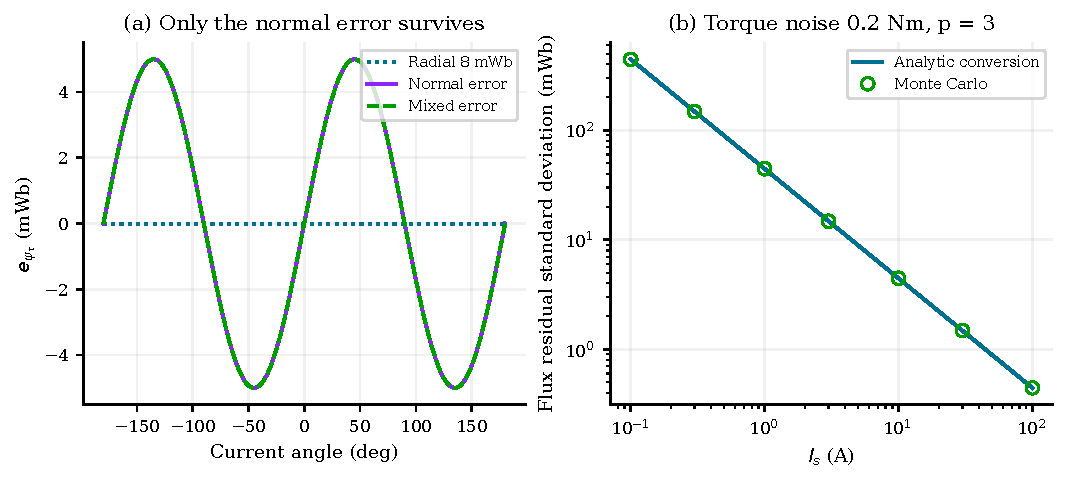
\includegraphics[width=\textwidth]{figures/07_torque_synthetic.pdf}
 \caption{Known-field numerical tests. Left: normal and mixed perturbations
 give the same normalized torque residual; a radial perturbation gives zero.
 Right: the original Monte Carlo noise checks agree with analytic
 $1/I_s$ amplification. Line patterns and open markers distinguish cases.}
 \label{fig:torque-synthetic}
\end{figure}

To test the interaction with reciprocity, use the dimensionless even
potential basis $[1,x,s,(x^2-y^2)/2,s^2]$, with
$x=i_d/I_*$, $y=i_q/I_*$, and $s=(x^2+y^2)/2$ on a full square grid.
Every candidate is reciprocal and has the required reflection.
Torque still annihilates the constant, $s$, and $s^2$ columns.
\Cref{tab:torque-rank} reports the generated ranks: voltage with known
resistance observes both radial slopes, and only the potential gauge remains.
Rows are dimensionless and scaled by $k_{\rm T}I_*\psi_*$ for torque and
$\omega_e\psi_*$ for voltage. These exact rank statements do not require
assuming equal real measurement uncertainties. Narrower current support
can lower rank further.

\begin{table}[htbp]
 \centering
 \begin{tabular}{lrr}
\toprule
Observation block & Rank & Nullity\\
\midrule
Torque & 2 & 3\\
Torque + voltage & 4 & 1\\
Torque + voltage + gauge & 5 & 0\\
\bottomrule
\end{tabular}

 \caption{Generated observation ranks for the five-column reciprocal,
 even potential example. Torque alone leaves two radial modes besides
 gauge; fixing gauge alone would not recover them.}
 \label{tab:torque-rank}
\end{table}

The original forty torque checks are retained, including weighted projection,
rotation, current noise, torque offset/gain, loss terms, resistance signs,
and joint rank. Additional tests cover both current axes, all quadrants,
both torque signs, the origin and small currents, reciprocal positive
isotropic inductance, the even-potential ranks, and excitation slices.
The pointwise projection is also checked to need not preserve conservation.
These are mathematical and implementation checks; no real-map correction
accuracy follows.

\section{Portable two-speed residual experiment}
\label{sec:real-torque}
The fixture \texttt{psm\_dual\_system\_multirpm} contains 218 operating
points: 109 each at requested 1000 and 3000 rpm, with a 70-$^\circ$C rotor
temperature reference and $p=4$. Flux reconstruction uses measured mean
electrical speed; requested speed only groups comparable conditions. Measured
and requested quantities are not interchanged.

\subsection{Configuration qualification precedes residual interpretation}
Selector 1 represents two amplitude-invariant three-phase systems. With equal
represented system currents, total electromagnetic torque is
\begin{equation}
 M_{\mathrm{total}}=2\left[\frac32p(\psid\iq-\psiq\id)\right],
 \qquad \kt=3p=12.
 \label{eq:dual-system-torque}
\end{equation}
The earlier single-system factor $3p/2=6$ omitted half the represented total;
using the recorded configuration reduces the combined uncentered discrepancy
RMS from 19.71 to \SI{1.21}{\newton\metre}. This is a necessary configuration
diagnosis, not a fitted gain or the contribution claimed by this paper.

The CAN channel is transported numerically without a calibration certificate,
known shaft location, gear ratio or loss map. Its comparison with model torque
is conditional. No torque outlier deletion is applied, and the small-current
threshold is used only for normalized legacy diagnostics, not for fitting the
global residual.

\subsection{Offset, structure and a common correction}
With $r_M=M_{\mathrm{CAN}}-M_{\mathrm{theo}}$, the 1000-rpm group has bias
$-0.876$ Nm, uncentered RMS $0.958$ Nm and centered RMS $0.386$ Nm. At
3000 rpm these values are $-1.331$, $1.427$ and $0.515$ Nm. Thus much of the
uncentered discrepancy is an admissible group offset, but centering does not
remove all spatial variation.

A quadratic low-complexity residual surface reduces five-fold spatial
cross-validation RMS to $0.334$ Nm at 1000 rpm, compared with the constant
model's $0.386$ Nm. At 3000 rpm it gives $0.515$ versus $0.515$ Nm. The first
slice therefore contains reproducible slow structure; evidence for that model
extension is weak in the second. This diagnostic does not decide whether the
structure comes from flux, losses, voltage reconstruction or torque sensing.

Fit one co-energy correction shared by both speeds and a separate $c_g$ per
speed, using fixed $\lambda=10$. Centered residual RMS becomes $0.317$ Nm at
1000 rpm and $0.458$ Nm at 3000 rpm, with a $0.728$ mWb RMS flux change.
These are in-sample consistency improvements and cannot validate true flux.

\begin{figure}[htbp]
 \centering
 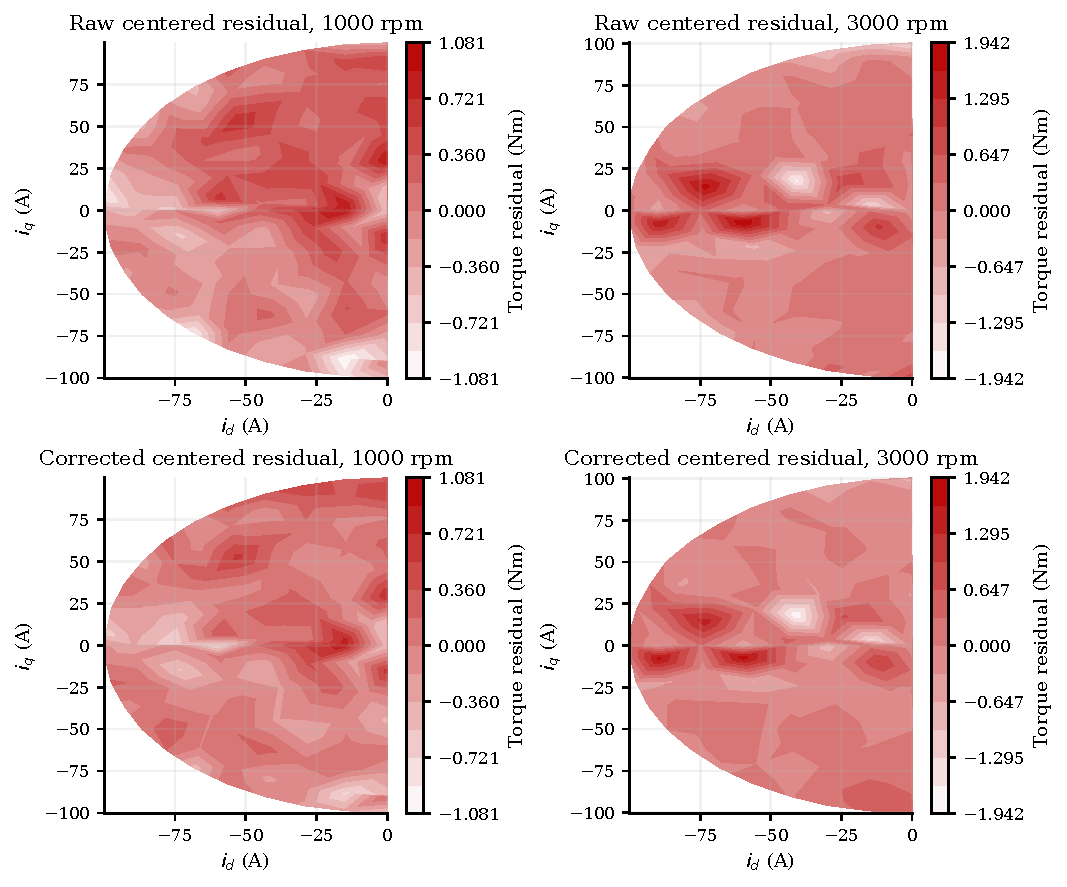
\includegraphics[width=\textwidth]{figures/09_real_residual_surfaces.pdf}
 \caption{Measured-minus-theoretical residual after subtracting each surface's
 group mean. The correction reduces some spatial structure but does not make the
 two speed slices equivalent. Color bars retain torque units.}
 \label{fig:real-residual-surfaces}
\end{figure}

\begin{figure}[htbp]
 \centering
 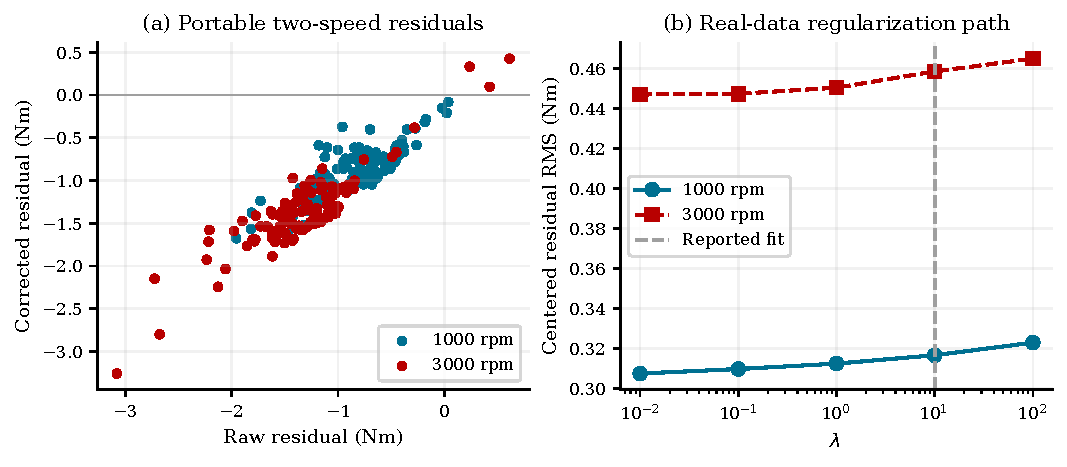
\includegraphics[width=\textwidth]{figures/10_real_regularization.pdf}
 \caption{Standalone two-speed summary. Left: raw and corrected residuals still
 include different nonzero offsets. Right: centered residual spread versus the
 declared regularization weight; no unknown real-flux RMSE is used for tuning.}
 \label{fig:real-regularization}
\end{figure}

\subsection{The decisive multi-speed transfer check}
A correction fitted only at 1000 rpm reduces its own centered residual but
increases the 3000-rpm spread; the converse fit likewise worsens 1000 rpm.
Consequently the available channel does not support interpreting either
single-speed fit as one speed-invariant magnetic correction. The joint fit is
a regularized descriptive compromise. Speed-dependent loss, voltage error,
sensor behavior or state mismatch remain plausible nuisance mechanisms.

Every operating point is written to \texttt{figures/data/real\_residuals.csv}
with raw and corrected flux, measured and theoretical torque, raw and corrected
residual, and the applied correction. The complete regularization path is a
second CSV; provenance, offsets, low-complexity diagnostics and transfer results
are stored in \texttt{numerics/real\_evaluation.json}.

\section{Relation to symmetry, reciprocity and multi-speed identification}
Reflection symmetry tests forbidden even/odd components and gives a closest
pair under a declared metric. It does not supply the independent torque shape
used here, and the present objective does not re-identify a winding resistance.
Quantities normalized under a sole resistance-mismatch hypothesis remain
\emph{resistance-equivalent} rather than physical resistance estimates.

Reciprocity asks whether a field can be the gradient of one co-energy surface.
The selected numerical correction satisfies that model structurally, but the
raw terminal reconstruction may contain nonconservative measurement effects.
Adding a curl-free correction cannot cancel their curl. Low torque residual,
low curl and smoothness are separate admissibility statements, not mutually
validating proofs of true flux.

Multi-speed data can test whether a proposed correction transfers across
conditions. A resistance-induced reconstruction error ideally scales with
$1/\omega_e$, whereas an ideal static magnetic map does not. Current-proportional
voltage error has the same column as resistance mismatch at every speed, and
terminal current need not equal the magnetic storage current in a loss-aware
model. The companion identifiability paper owns the scaled rank, nuisance and
support analysis. This paper uses its conclusion operationally: a correction
that helps one speed but harms another is evidence against a common magnetic
interpretation under the current nuisance model.

\section{Interpretation after the configuration check}
\label{sec:torque-ambiguity-discussion}
Torque observes a normal projection and leaves a radial slope free. Adding
a smooth radial potential can preserve reflection, reciprocity and positive
curvature while leaving every torque value unchanged. Zero discrepancy is
therefore insufficient for full flux reconstruction, even with an ideal sensor.
Pointwise minimum change chooses a representative; it need not retain curl-free
structure across the current plane.

The six-phase interpretation resolves the leading scale disagreement in the
real case. It does not qualify the independent CAN observation as electromagnetic
truth. If its shaft meaning were established, the signed rotor balance would be
\begin{equation}
 \rotorinertia\dot{\mechanicalspeed}
 =M_{\rm em}-\shafttorque-\mechanicallosstorque.
 \label{eq:shaft-torque-balance}
\end{equation}
Even at steady speed mechanical losses separate transmitted and electromagnetic
torque. Equal represented system currents, matched acquisition windows and
terminal-voltage meaning are additional requirements. Sensor offset produces
inverse-current amplification, gain a torque-proportional term, and current
bias changes both the map argument and lever arm. A coherent common rotation
preserves oriented area, while inconsistent frames can change it.

The synthetic ranks apply to their stated operators and support. Real
joint electrical-mechanical estimation needs covariance, parameter scaling
and nuisance columns. A radial magnetic or electrical observation remains
necessary even after the torque channel is fully qualified.

\section{Conclusion}
Independent torque measures one local flux projection, leaving a radial
solution family. Smooth reciprocal and reflection-preserving radial potentials
show why magnetic constraints do not generally close that ambiguity.
The portable real study identifies a missing two-system torque contribution
from recorded six-phase configuration and substantially reduces the CAN
discrepancy without calibration fitting. The remaining comparison retains
its sensor and mechanical qualifications; the data do not justify a full
magnetic correction or complete flux reconstruction.


\ifshowglossary
  \glsadd{pmsm}\glsadd{dq}
  \glsadd{sym:id}\glsadd{sym:iq}\glsadd{sym:rs}\glsadd{sym:omega}
  \glsadd{sym:coenergy}
  \glsadd{sym:stationarytorqueresidual}\glsadd{sym:torquegroupoffset}
  \printnoidxglossary[type=\acronymtype,title={Acronyms}]
  \printnoidxglossary[type=symbols,title={Symbols}]
\fi
\ifshowbibliography
  \printbibliography
\fi
\end{document}
